\documentclass{article}
\usepackage[utf8]{inputenc}
\documentclass[french,12pt]{report}
%Some packages I commonly use.
%\usepackage[english]{babel}
\usepackage[french]{babel}
\usepackage{graphicx}
\usepackage{framed}
\usepackage[normalem]{ulem}
\usepackage{amsmath}
\usepackage{amsthm}
\usepackage{amssymb}
\usepackage{amsfonts}
\usepackage{enumerate}
\usepackage{xcolor}
\usepackage[utf8]{inputenc}
\usepackage[top=1 in,bottom=1in, left=1 in, right=1 in]{geometry}
\usepackage{systeme}
\usepackage{hyperref} 
\usepackage{dsfont}
\usepackage[


\begin{document}

\textbf{\textit{Introduction}} \\  \\


Les modèles linéaires à effets mixtes (LMM) sont devenus l'outil de choix pour analyser les données dépendantes Contrairement aux modèles linéaires standard, les modèles LMM font des hypothèses non seulement sur la distribution des résidus, mais aussi sur la distribution des effets aléatoires .Malheureusement, les hypothèses de distribution des effets aléatoires ne peuvent pas être vérifiées aussi facilement que pour les effets fixes .
Officiellement, les hypothèses d'un modèle à effets mixtes impliquent la validité du modèle, l'indépendance des points de données, la linéarité de la relation entre le prédicteur et la réponse, l'absence d'erreur de mesure dans le prédicteur, l'homogénéité des résidus, la dépendance des effets aléatoires par rapport aux covariables (exogénéité), l'absence totale de données au hasard et des hypothèses sur la distribution des résidus et des effets aléatoires . \\

 Une autre façon d'énoncer les hypothèses de base est que les résidus et les coefficients d'effets aléatoires sont indépendants et distribués de manière identique. Toute violation de ce principe implique l'invalidité du modèle. Et donc le modèle doit être complet de telle sorte que tous les effets restants soient marginalisés par une randomisation appropriée. Les modèles mixtes sont en général  flexibles dans leurs utilisation des distributions variables . On note que les distributions normales sont de loin les plus utilisées. Une autre problématique est de savoir si les violations de l'hypothèse de normalité affectent l'ajustement du modèle. \\ 
Le diagnostic du modèle est généralement basé sur l'évaluation de la distribution des résidus de Cholesky .Normalement, les résidus doivent être distribués suivant la loi Normale  bien qu'une distribution normale des résidus ne garantisse pas que les hypothèses de distribution soient remplies. On peut alors essayer d’évaluer  l'hétéroscédasticité. Toutefois, à la différence des modèles linéaires standard, les hypothèses de distribution des modèles à effets mixtes doivent être vérifiées à plusieurs niveaux, y compris la distribution des coefficients d'effets aléatoires .
Les hypothèses de distribution sont en général difficiles à vérifier, en particulier en ce qui concerne les effets aléatoires. \\
On note aussi que due au fait que les moyennes des groupes ne sont pas observables particulièrement pour les modèles linéaires généralisés à effets mixtes, les violations peuvent être causées par des violations de la distribution des effets aléatoires ou d'autres parties du modèle .En conséquence, McCulloch et Neuhaus (2011) ont suggéré de vérifier d'abord les hypothèses de distribution des niveaux inférieurs, avant de vérifier la distribution des niveaux de groupe. Une vérification postérieure du modèle prédictif offre une approche générale pour vérifier l'exactitude prédictive d'un modèle. Un contrôle à posteriori du modèle prédictif est basé sur la simulation des données à l'aide d'estimations des paramètres du modèle tout en intégrant l'incertitude dans les estimations et des mesures pertinentes pour évaluer si les valeurs observées se situent dans la fourchette des valeurs simulées. Le problème avec cette approche est que le choix des caractéristiques pertinentes pour l'évaluation peut être difficile à établir. On ne peut pas donc limiter notre choix sur  La valeur moyenne d'un paramètre , mais d'autres aspects de la distribution des observations, tels que l'occurrence de valeurs extrêmes, peuvent l'être.\\ 



Les effets fixes se sont avérés largement résistants aux violations des hypothèses de distribution des effets aléatoires, du moins pour les modèles gaussiens. Pour les modèles linéaires généralisés à effets mixtes, les modèles ont été plus variables et les estimations des effets fixes peuvent être biaisées dans certains cas. Dans l'ensemble, les violations des hypothèses concernant les distributions d'effets aléatoires semblent avoir des conséquences mineures pour les modèles linéaires, mais peuvent avoir des conséquences graves pour les modèles non linéaires, y compris les modèles linéaires généralisés à effets mixtes . L'estimation de la variance du groupe est généralement exacte, mais les coefficients des effets aléatoires  sont souvent mal estimés. \\
L’article aborde plusieurs questions générales sur la robustesse des MPC aux violations des hypothèses de distribution à chaque niveau d'un modèle et se concentre sur les estimations des paramètres, c'est-à-dire les pentes pour les effets fixes et la variance expliquée par les effets aléatoires, qui sont généralement du plus grand intérêt pour les chercheurs en écologie et en évolution. Certaines simulations présentent plusieurs violations graves des hypothèses de distribution, notamment des distributions biaisées, bimodales et hétéroscédastiques des résidus, ainsi que des composantes d'effets aléatoires manquantes. De telles violations des hypothèses de distribution peuvent survenir pour diverses raisons dans des ensembles de données réelles, par exemple si une influence pertinente (comme l'état d'un organisme ou le moment de l'échantillonnage) n'est pas prise en compte ou si les mesures montrent des effets limites. Les violations des hypothèses de distribution de la variance d'erreur et de la distribution des effets aléatoires permettent d’évaluer l'effet sur les estimations des paramètres. Dans l'ensemble, il s’agit d’une robustesse remarquable des LMM. Le biais est généralement faible dans les paramètres estimés, les problèmes les plus prononcés survenant lorsque les prédicteurs ou les composantes des effets aléatoires sont absents. Une exploration superficielle des modèles linéaires généralisés à effets mixtes (MLM) montre une robustesse substantielle également, mais aussi quelques complications notables. \\ 







\textbf{\textit{Modèle de base simulé}}\\

La première partie de l’étude consiste à simuler des données et à les ajuster dans un simple LMM, puis à enfreindre les hypothèses sur les effets aléatoires et les distributions d'erreurs. \\
Le modèle de base contenait deux prédicteurs à effets fixes continus tirés de normes non corrélées et les distributions avec une moyenne nulle et une variance unitaire. 

la pente de la variable de réponse sur chacune de ces covariables ($x_1$ et $x_2$) a été fixée à $+0,2$ pour l'effet fixe d'intérêt $\beta_1$  et à $-0,2$ pour le second effet fixe $\beta_2$. \\

 Comme les covariables sont centrées et que leurs pentes sont de signes opposés, leurs effet global attendu sur la moyenne est nul. \\

120 observations ont été généré par itération puis ont été regroupées en 30 groupes. Le nombre de répétitions par groupe a varié, et chaque groupe est représenté au moins une fois. Cela permet de simuler un échantillonnage déséquilibré. Des moyennes au niveau des groupes ainsi que des écarts résiduels ont été tiré à partir d'une distribution normale avec une moyenne de zéro et une variance de 0,5. 



$$ y=\beta_0+\beta1x_1+\beta_2x_2+\alpha+\epsilon  $$
$$ \alpha \sim  N(0,\sigma^2_{\alpha}) $$
$$ \epsilon \sim  N(0,\sigma^2_{\epsilon}) $$

où y est un vecteur de la réponse simulée, $\beta_0$ est l'interception qui a été fixée à 1, $x_1$ et $x_2$ sont les vecteurs des valeurs des covariables, $\beta_1$ et $\beta_2$ sont les deux pentes qui ont été fixées à :  $\beta_1 = 0,2$ et $\beta_2 = -0,2$, respectivement,
$\alpha$ représente un vecteur de l'effet aléatoire pour l'identité de groupe, $\epsilon$ vecteur
des erreurs résiduelles, $\sigma^2_{\alpha}$ la variance entre les groupes (fixée à 0,5)
et $\sigma^2_{\epsilon}$ la variance des erreurs (variance intra-groupe, fixée à 0,5).  \\
La variance phénotypique prévue était 
\begin{center}

$\sigma^2_{p}=\sigma^2_{\alpha}+\sigma^2_{\epsilon}+\beta^2_{1} \sigma^2_{x_1} +  \beta^2_{2} \sigma^2_{x_2}=1.08$ \\

\end{center}

\textbf{\textit{Modèles de référence}} \\
\\
10 000 ensembles de données simulées sont générées puis ajusté suivant le modèle d'analyse :

$$ y=\beta_0+\beta_1 x_1+\beta_2x_2+\hat{\alpha}+\hat{\epsilon}  $$
$$ \hat{\alpha} \sim  N(0,\hat{\sigma}^2_{\hat{\alpha}}) $$
$$ \hat{\epsilon} \sim  N(0,\hat{\sigma}^2_{\hat{\epsilon}}) $$

avec $\hat{\beta_0},\hat{\beta_1},\hat{\beta_2},\hat{\alpha},\hat{\epsilon}$     sont respectivement les approximations de :  $\beta_0,\beta_1,\beta_2,\alpha,\beta$. \\
Les models ont été volentairement mal spécifié dans les hypothèses de répartition, en ignorant les indicateurs de performance, la structure de regroupement ou les corrélations entre les prédicteurs. \\
 La pente b a été estimée  vis à vis des differents paramètres puis le biais  comme étant l'écart moyen par rapport à la valeur simulée, puis l'erreur de prédiction comme étant la racine carrée des écarts moyens au carré de l'estimation par rapport à la valeur simulée (erreur quadratique moyenne, EQM). 

$${\displaystyle \operatorname {MSE} ({\hat {\theta }})\,{\overset {\text{def}}{=}}\,\mathbb {E} \left[({\hat {\theta }}-\theta )^{2}\right]}$$


L’analyse est axée sur l'estimation et moins sur les erreurs d'inférence, car la chronologie de la taille de l'effet est la plus pertinente à long terme. 
\\ \\
\textit{\textbf{Violations des hypothèses de répartition}} \\  \\
L'analyse des données à l'aide des LMM suppose généralement que $\alpha$ et $\epsilon$ sont échantillonnés à partir de distributions normales comme dans nos simulations de base ci-dessus. Pour évaluer si la violation de cette hypothèse pose problème, elle a été volontairement non respectée en simulant des ensembles de données dans lesquels les échantillons  $\alpha$ et $\epsilon$ ont été choisis à partir d'autres distributions. Cela a été fait indépendamment pour les deux termes :  un à la fois puis les deux en combinaison. \\
 
 \textbf{\textit{Distributions biaisées (scénarios A)}} : Au lieu de prendre des distributions normales standard,  $\alpha$ et $\epsilon$ ont été tirés des distributions biaisées.
\\ \\

\textbf{\textit{Distributions bimodales (scénarios B) }}: les distributions ont été tirées de deux distributions normales distinctes avec les moyennes déplacées ±1,5 unités. Le décalage a été fait au hasard, de sorte qu'environ la moitié des tirages soit déplacée vers le bas et la moitié vers le haut. Cela a donné des distributions bimodales.L'ajout de modes décalés affecte la variance résiduelle totale simulée. Afin d'ajuster le niveau du groupe et la variance résiduelle à la valeur cible, la variance a été  réajustée. \\ \\\

\textbf{\textit{Distributions hétéroscédastiques (scénarios C) :}}  $\alpha$ et $\epsilon$  sont tirées de distributions où la variance dépend d'une des covariables (x1) tq : 

$$\sigma^2_{Het}=\sigma^2 + \lambda(X_1-min(x_1)) $$
où le facteur d'hétéroscédasticité $\lambda$  prend les valeurs 2, 4 ou 8. \\
On note qu’un facteur d'hétéroscédasticité de 0 donne la distribution normale standard et un facteur d'hétéroscédasticité de 8 garantissent que l'hétéroscédasticité est extrême, probablement plus que dans la plupart des applications réelles afin de découvrir même les petits biais. L'incorporation d'un paramètre d'hétéroscédasticité affecte la variance résiduelle totale simulée. Afin de redimensionner la variance résiduelle à la valeur cible, il faut rétablir l'écart, notament en utilisant : $$ \epsilon=\epsilon'\frac{\sqrt{\sigma^2_\epsilon	}}{SD(\epsilon')}$$
où $\epsilon$ est l'erreur résiduelle après addition du facteur d'hétéroscédasticité, $SD(\epsilon′)$ est l'écart-type de $\epsilon′$ et $\sigma^2_\epsilon$est la variance résiduelle cible fixée à 0,5. \\ 

 \textbf{\textit{Effets aléatoires manquants (scénarios D)}} 
Afin d'étudier les effets aléatoires manquants,  3 effets aléatoires ont été introduit : \\
Un effet aléatoire de niveau supérieur (avec dix niveaux), un effet aléatoire de niveau inférieur (avec 60 niveaux) et un effet aléatoire croisé (avec 30 niveaux  ). D'autres effets aléatoires ont été échantillonnés de manière aléatoire, c'est-à-dire de manière déséquilibrée, en veillant à ce que chaque groupe soit représenté au moins une fois.

Les variances à effet aléatoire ont été fixées à $\sigma^2_H = 0,5$ pour l'effet aléatoire de niveau supérieur, $\sigma^2_L = 0,5$ pour l’inférieur et $\sigma^2_C = 0,5$ pour l'effet aléatoire croisé, tandis que la variance de l'effet aléatoire d'intérêt et la variance résiduelle ont été conservés à $\sigma^2_\alpha = 0,5$ et $\sigma^2_\epsilon = 0,5$  \\ 

\textbf{\textit{Prédicteurs corrélés(scénarios E)}}

La version de base du modèle a généré des valeurs de covariables indépendantes. Des cas de prédicteurs corrélés on été introduit en tirant les valeurs des covariables $x_1$ et $x_2$ de distributions normales multivariées avec des corrélations fixées à +0,2, +0,5 ou +0,8 . Ces simulations ont été introduites pour étudier les biais et les erreurs de prédiction dans une situation généralement considérée comme problématique. Les trois valeurs de corrélation ont été choisies pour montrer l'effet des corrélations légères, modérées et fortes entre les prédicteurs. Au moins la situation avec une corrélation de 0,8 sera typiquement considérée comme très problématique. \\

\\    
\textbf{\textit{Résultats : }}
\\ \\

On note que pour la première figure qui traite  les effets des violations des hypothèses de distribution sur les estimations des paramètres d'intérêt majeur; la rangée supérieure correspond au modèle mixte de base avec groupe normal et variances résiduelles, la deuxième rangée correspond à la distribution biaisée des variances résiduelles, et la troisième correspond à la distribution biaisée des variances de groupe et finalement la dernière correspond à la distributions biaisées des écarts de groupe et des écarts résiduels \\

\begin{center}
\textbf{\textit{Violation en biais}}
\end{center}

         $$  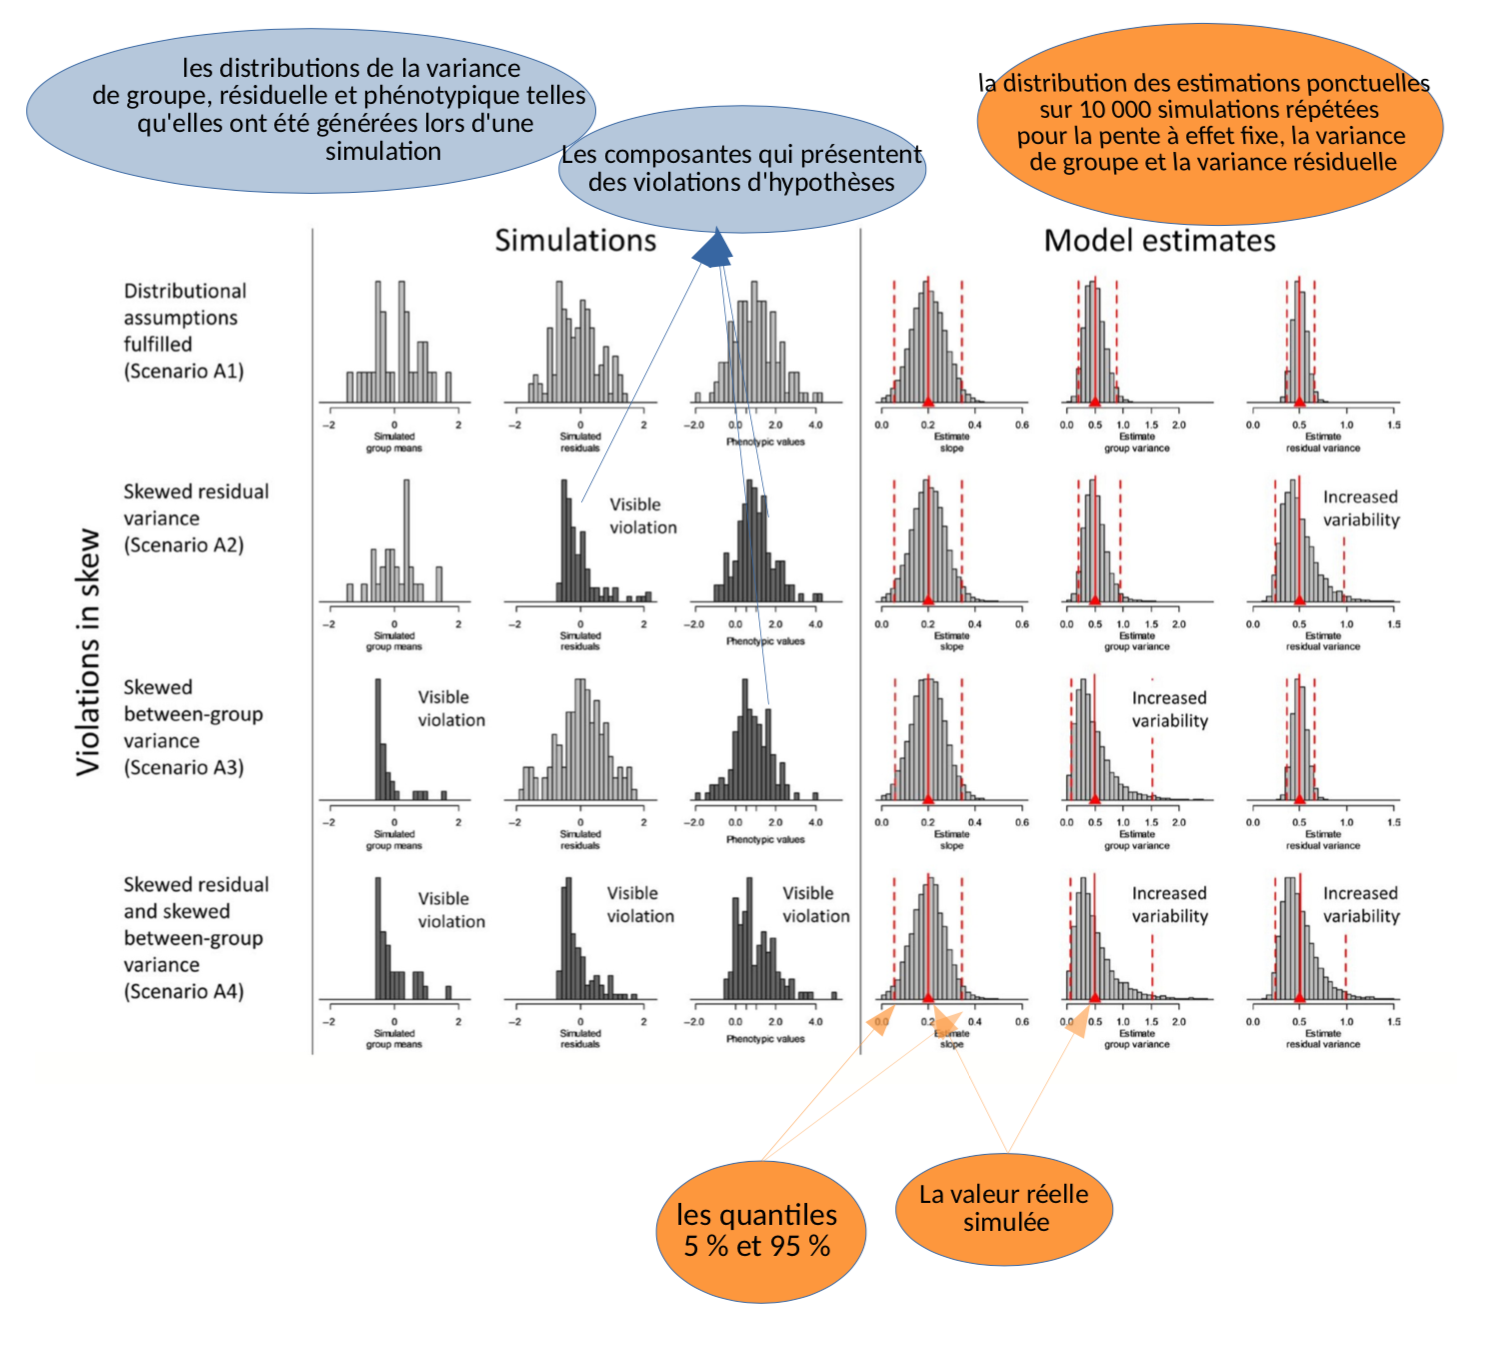
\includegraphics[scale=0.6]{11.png} $$\textbf{\textit{Figure 2 : }}
        La deuxième figure traite les effets des distributions biaisées et de la taille des composantes de la variance sur les moyennes et les résidus estimés des groupes. 


$$  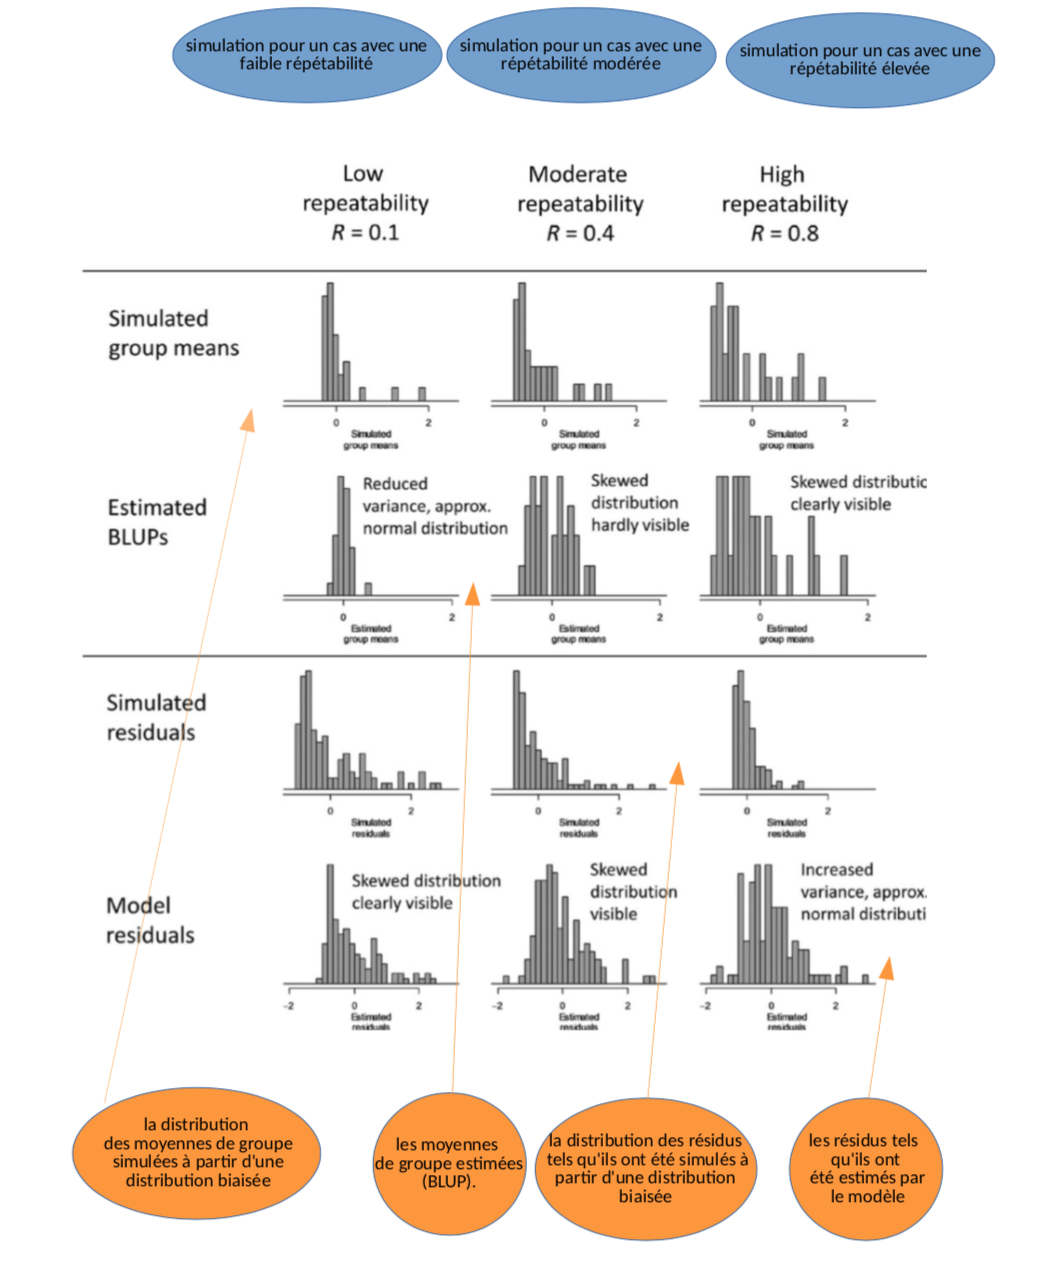
\includegraphics[scale=0.7]{2p.png} $$
\textbf{\textit{Figure 3 : }}

La figure 3 traite les impactes des effets aléatoires manquants sur les estimations des paramètres d'intérêt : 


$$  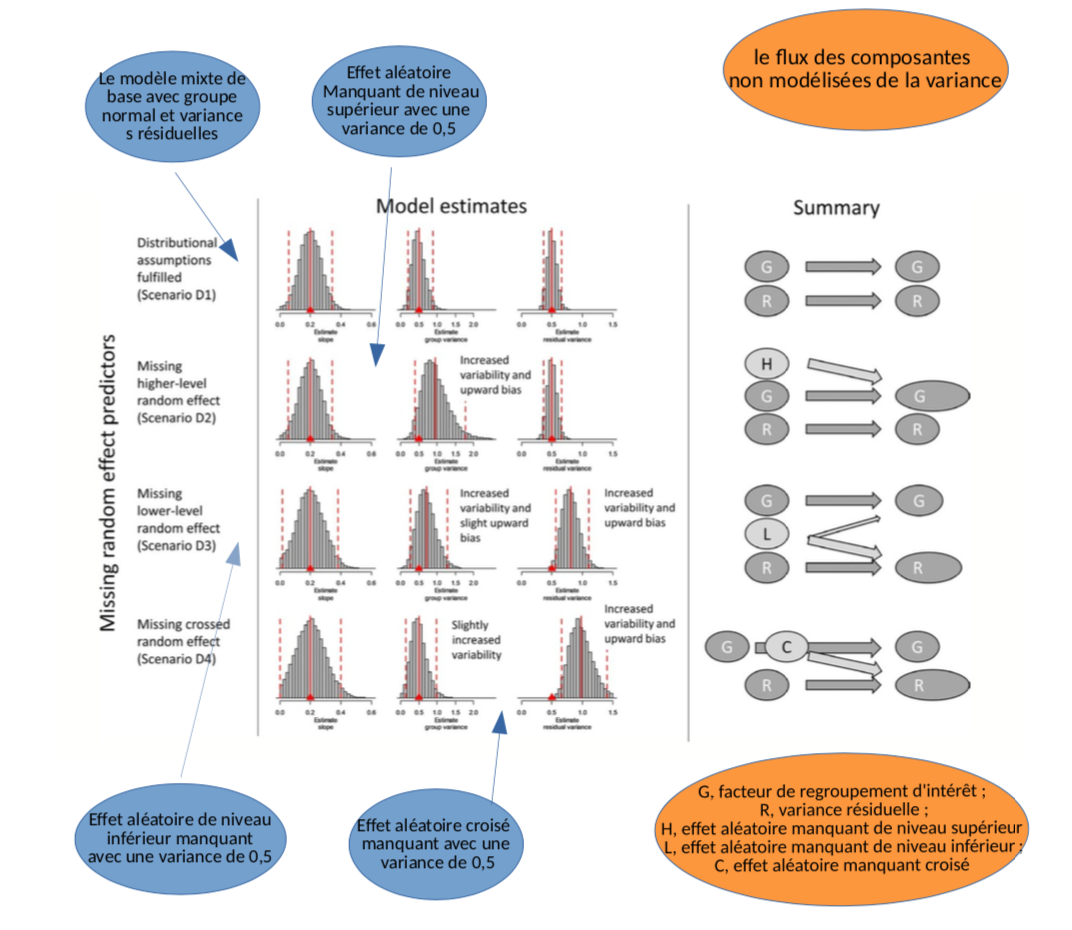
\includegraphics[scale=0.7]{4.png} $$\textbf{\textit{Figure 4 : }}


$$  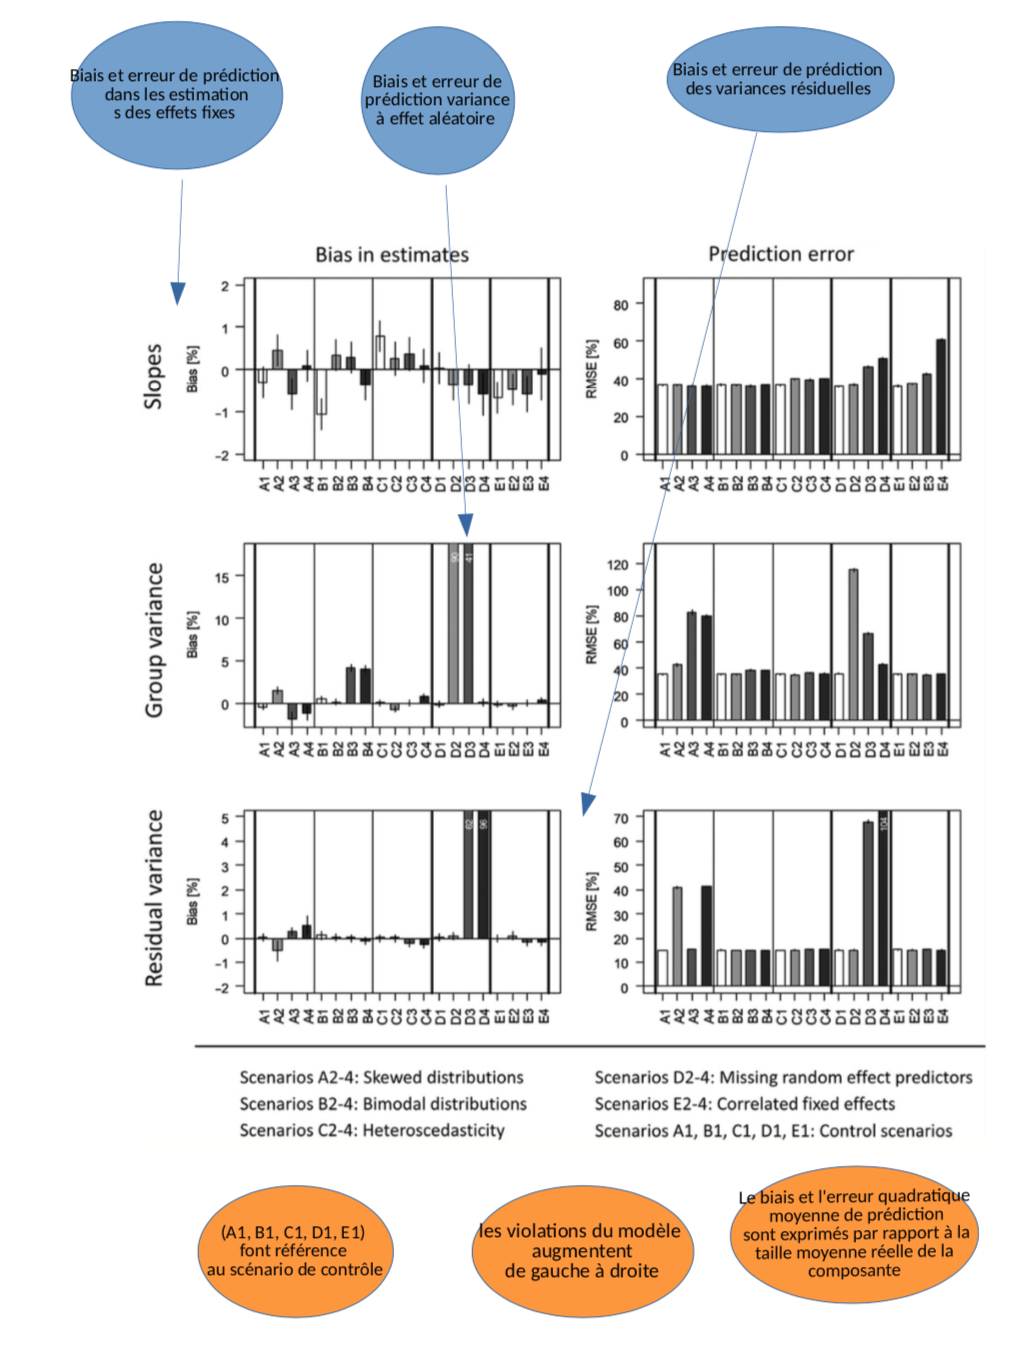
\includegraphics[scale=0.7]{5p.png} $$


\textbf{\textit{Analyse : }}
\\ \\
L’analyse de simulation montre que l'effet des violations des hypothèses de distribution des variances à effet aléatoire et des résidus est étonnamment faible. Même les distributions bimodales et hétéroscédastiques fortement biaisées ont entraîné un faible biais global, à l'exception des variances de groupe estimées pour les données générées à partir d'une distribution bimodale. Les estimations à effet fixe sont peu biaisées, bien que la couverture des intervalles de confiance soit trop faible dans le cas des variances résiduelles hétérogènes. Cependant, les composantes de la variance pour lesquelles l'hypothèse de normalité est vérifiée présente une erreur de prédiction significativement plus élevée, ce qui signifie que les estimations sont plus variables et donc moins précises. \\

Par conséquent, bien que les estimations ne soient pas biaisées en moyenne, elles peuvent être plus éloignées de la valeur réelle que lorsque les hypothèses de distribution ne sont pas remplies.\\ 
Certaines des violations simulées pourraient facilement émerger de modèles incomplets. Les distributions bimodales, par exemple, peuvent souvent résulter d'un fort effet d'une variable de classe qui n’a pas été incluse dans le modèle. En effet, c'est ainsi que les distributions bimodales ont été généré dans la simulation. L'identification et l'ajustement des effets manquants permettent de stabiliser les distributions et donc d'améliorer les estimations. Des effets similaires peuvent sous-entendre les cas d'hétéroscédasticité.\\

 On note que les distributions biaisées résultent souvent d'effets multiplicatifs plutôt qu'additifs. Il convient donc d'évaluer l'échelle de la mesure dans de tels cas.\\

Aussi  les termes d'effet aléatoire manquants ont des effets systématiques sur les estimations d'autres composantes de la variance. Les sources de variance non modélisées ont des effets prévisibles sur les composantes de variance du modèle qui dépendent de la structure hiérarchique de l'ensemble de données. Ces effets sont analogues à une cascade, où les variances descendent dans la hiérarchie, mais ne montent généralement pas. Par conséquent, les variances de la structure manquante de niveau supérieur descendent en cascade vers un effet aléatoire de niveau inférieur qui est inclus dans le modèle. Et donc les effets aléatoires de niveau inférieur et de niveau égal descendent en cascade jusqu'aux résidus. Cela implique également que, face au problème de l'incitation à omettre l'un des deux effets aléatoires hiérarchiques, c'est généralement l'effet aléatoire de niveau inférieur qui doit être modélisé et l'effet aléatoire de niveau supérieur qui est omis. Ce problème peut apparaître dans des modèles très complexes, par exemple le cas où deux niveaux sont presque identiques dans leurs niveaux de facteurs. Il est alors préférable de modéliser l'effet aléatoire avec plus de niveaux. \\

Il reste une imprécision accrue des estimations d'effets fixes lorsque les covariables sont corrélées. Les avertissements concernant les effets fixes corrélés sont nombreux. En general, les effets importants sur la précision des estimations n'est évident que dans le cas des fortes corrélations. Tandis que pour les corrélations faibles et modérées, elles ont très peu d'effet. Ainsi  si la corrélation entre les prédicteurs affecte les estimations des variables impliquées dans ces corrélations, le problème ne se répercute pas sur le reste du modèle, c'est-à-dire qu'il n'affecte pas les estimations des composantes à effet aléatoire ou d'autres prédicteurs non corrélés.\\


Une autre problématique concernant les estimations très variables est de savoir si l'incertitude est correctement reflétée dans l'erreur type des estimations. Les estimations à effet fixe n'ont pas montré de niveaux élevés d'imprécision contrairement à l'estimation de l'incertitude pour la variance à effet aléatoire. Toutefois, il n'existe pas de méthode universellement acceptée pour quantifier l'incertitude des variances à effet aléatoire. Les probabilités de profil, l'estimation bayésienne ou le bootstrapping paramétrique offrent trois options très différentes. Les résultats des simulations donnent quelques indications sur la manière dont le bootstrapping paramétrique est susceptible de fonctionner. Le bootstrapping paramétrique repose sur des simulations basées sur des estimations du modèle, suivies d'un réajustement du modèle et d'une évaluation de la variabilité des estimations d'une simulation à l'autre. Dans le cadre de l’article le bootstrap ne couvre pas bien les estimateurs corrects et pour ça il n’a pas été utilisé. On note que toutes les méthodes échoueront probablement à prédire avec précision les niveaux d'effets aléatoires spécifiques.\\


Une pratique courante consiste à effectuer des transformations non linéaires de la variable de réponse afin d'améliorer l'ajustement aux distributions normales. Toutefois quand les données  ne sont pas à l'échelle originale cela se fait au prix d'une interprétation réduite, et dans le cadre de l’article, l'hypothèse de normalité n’est pas respectée,  et donc les transformations pourraient ne pas être nécessaires. Il est donc avantageux d'éviter la transformation face au compromis entre l'interprétabilité et la conformité aux hypothèses du modèle. \\



Les simulations suggèrent que l'estimation de la pente est pertinente, et donc le gradient de sélection sera probablement non biaisée.\\
Les résultats obtenus dans l’article montrent une robustesse remarquable, même avec des données non équilibrées. \\

Dans la simulation effectuée dans l’article, l’étude des distributions d'erreurs non gaussiennes a été faite de façon assez superficielle. Les distributions gaussiennes peuvent être modélisées par des modèles linéaires généralisés à effets mixtes (MLGM). Les MLG comprennent des fonctions de liaison et des distributions d'erreurs spécifiques. L'éventail des options possibles est vaste, les GLMM de Poisson, les GLMM binomiaux et les GLMM négatifs-binomiaux étant les plus populaires. La fonction de liaison et les distributions d'erreurs spécifiques entraînent des complications supplémentaires et doivent être choisies de manière appropriée. Toutefois, à l'échelle latente, les modèles sont équivalents aux GLMM gaussiens, de sorte que la plupart des résultats s'appliqueront probablement aussi aux GLMM non gaussiens. Les simulations pour les données de Poisson et de proportion indiquent que les résultats sont globalement similaires, mais les modèles de Poisson et binomiaux se répandent différemment en fonction des violations dans différentes situations. La robustesse semble donc être beaucoup plus spécifique au contexte dans le cas des GLMM. En outre, la réponse attendue dépendra également de la valeur moyenne de la population. Pour la simulation de MGML binomiales, nous avons choisi une moyenne de zéro sur l'échelle latente, ce qui donne une réponse attendue moyenne de 0,5 sur l'échelle observée et donc une information maximale par point de données. D'autres cas peuvent être moins favorables. \\

En raison du faible impact de l'hétéroscédasticité sur les estimations du modèle, il ne semble pas nécessaire d'ajuster les variances résiduelles hétérogènes lorsque l'objectif principal est d'obtenir des estimations robustes des composantes à effets fixes et aléatoires dans la partie fixe du modèle. Les dHGLM font des hypothèses supplémentaires qui nécessiteront des vérifications supplémentaires. \\
Dans de nombreux cas, une partie de la spécification du modèle approprié devrait inclure des termes de pente aléatoire lorsque les données sur les pentes sont reproduites au sein de groupes. Les modèles à pentes aléatoires peuvent se compliquer, en particulier si plusieurs termes à pentes aléatoires doivent être inclus. En général, une attention particulière est nécessaire pour que les modèles continuent à fournir des estimations appropriées. \\

Il est possible que les violations des distributions d'effets aléatoires qui sont impliquées dans les termes de pente aléatoire puissent causer des estimations biaisées et/ou imprécises. Les simulations de modèles à pente aléatoire avec violation de la distribution des effets aléatoires suggèrent la robustesse du taux d'erreur de type 1 à effet fixe si la variance de la pente aléatoire est spécifiée de manière appropriée , mais les conditions dans lesquelles les pentes aléatoires ne sont pas spécifiées de manière appropriée sont largement inexplorées. \\



\textbf{\textit{Résumé:}} \\  \\

Les modèles d'effets linéaires mixtes sont des outils puissants pour analyser des ensembles de données complexes avec des observations répétées ou groupées. Ils impliquent des procédures d'ajustement complexes et font plusieurs hypothèses, en particulier sur la distribution des effets résiduels et aléatoires. \\ 
 Les violations de ces hypothèses sont courantes dans les ensembles de données réels, mais il n'est pas toujours évident de savoir dans quelle mesure ces violations sont importantes pour une estimation précise et impartiale.\\
On va traiter les conséquences des violations des hypothèses de distribution et l'impact des composantes manquantes des effets aléatoires sur les estimations du modèle. En particulier, nous évaluons les resultats de l'effet aléatoire et des variances latérales biaisées, bimodales et hétéroscédastiques, des termes d'effet aléatoire manquants et des prédicteurs à effet fixe corrélés. Pour cela nous allons nous concentrer sur le biais et l'erreur de prédiction sur les estimations des effets fixes et aléatoires.\\ 

Les estimations des modèles sont généralement robustes face aux violations d'hypothèses, à l'exception d’une hausse légère du biais dans les estimations de la variance des effets aléatoires. En outre, les estimations des composantes à effet aléatoire qui enfreignent les hypothèses de distribution deviennent moins précises mais restent non biaisées. Cela a été également constaté pour les effets fixes fortement corrélés, ce qui a conduit à des estimations imprécises, mais non biaisées.\\

Des sources non modélisées de variance à effet aléatoire ont eu des effets prévisibles sur les estimations des composantes variables. On peut considérer le modèle comme une cascade de composantes hiérarchiques.\\

 Les écarts se répandent dans la hiérarchie de sorte que les écarts à effet aléatoire manquants de niveau supérieur se regroupent aux niveaux inférieurs et que les écarts à effet aléatoire manquants de niveau inférieur et croisés se manifestent sous la forme d'un écart résiduel.\\
Dans l'ensemble, les résultats de l’article montrent une remarquable robustesse des modèles à effets mixtes qui devrait permettre aux chercheurs d'utiliser des modèles à effets mixtes même si les hypothèses de distribution sont objectivement violées. Toutefois, cela ne dispense pas les chercheurs d'évaluer soigneusement le modèle. Les estimations basées sur des données qui montrent des violations évidentes d'hypothèses clés doivent être traitées avec prudence car les ensembles de données individuels peuvent donner des estimations très imprécises, même si elles sont en moyenne non biaisées entre les ensembles de données. \\ \\

 \\  \\
        
  

  
\textbf{\textit{  Conclusion :}} \\ \\


Dans l'ensemble, les résultats trouvés dans l’article peuvent être considérés comme encourageants et permettent aux utilisateurs de modèles à effets mixtes d'avancer avec confiance. Les modèles à effets mixtes sont largement robustes, même s'ils ne respectent pas complètement les hypothèses du modèle. Bien qu'il puisse être intéressant de modéliser des données qui ne sont clairement pas normalement distribuées, nous mettons en garde contre le fait que cela pourrait entraîner une variabilité accrue des estimations, et donc des résultats extrêmes et donc trompeurs pour des ensembles de données spécifiques. \\ 

Cependant, l'effet est largement limité aux paramètres qui sont le plus étroitement liés aux violations des hypothèses. Il sera donc relativement facile d'identifier les estimations qui doivent être traitées avec une prudence accrue. Les résultats n'éliminent donc pas la nécessité d'une évaluation correcte de chaque modèle. Les contrôles de modèles prédictifs a posteriori semblent les plus adaptés. Toutefois, les modèles à effets mixtes ne doivent pas être considérés comme dangereusement compliqués. Il s'agit plutôt d'outils puissants permettant de modéliser une grande variété d'ensembles de données et ils sont généralement plus performants que les analyses alternatives.\\
Il peut donc être pratique d’utiliser des modèles à effets mixtes même pour des ensembles de données légèrement non standard, tout en préconisant des efforts visant à ne pas tenir compte des conséquences spécifiques de certains types de violations.

\end{document}
